\chapter{Planejamento do Experimento}\label{chapter:experimento}

Neste capítulo é apresentado o experimento que será realizado para a avaliação da proposta apresentada no Capítulo \ref{chapter:proposta}.
Para avaliar a proposta deste trabalho irá utilizar uma avaliação pela perspectiva do usuário, que segundo a definição de
\citeonline{shani2011evaluating} se encaixa em um Estudo com usuários. O algoritmo proposto será incorporado ao ambiente
AdaptWeb\textsuperscript e avaliado em uma situação real de uso em um minicurso de algoritmos. Esse capítulo explica
em mais detalhes o ambiente AdaptWeb\textsuperscript, as mudanças propostas para o ambiente e o experimento planejado.

\section{Descrição do Ambiente \adaptweb}

O \adaptweb (Ambiente de Ensino-Aprendizagem Adaptativo na Web) é um sistema open source
que consiste em um AVA capaz de adaptar o conteúdo, a apresentação e a navegação em determinado curso às características
e preferências do aluno \cite{gasparini2009adaptweb}. A Subseção \ref{subsection:estrutura-adaptweb} apresenta a Estrutura Geral do
\adaptweb.

\subsection{Estrutura do \adaptweb}\label{subsection:estrutura-adaptweb}

A estrutura do \adaptweb é composta por quatro módulos: (1) o módulo de autoria; (2) o
módulo de armazenamento em XML (Extensible Markup Language); (3) o módulo de adaptação do conteúdo baseado no modelo do
usuário e (4) o módulo de interface adaptativa \cite{gasparini2003interface}, conforme pode ser visto na Figura
\ref{fig:adaptweb-arquitetura}.

\begin{figure}[htb]
  \caption{\label{fig:adaptweb-arquitetura}Estrutura do \adaptweb}
  \begin{center}
      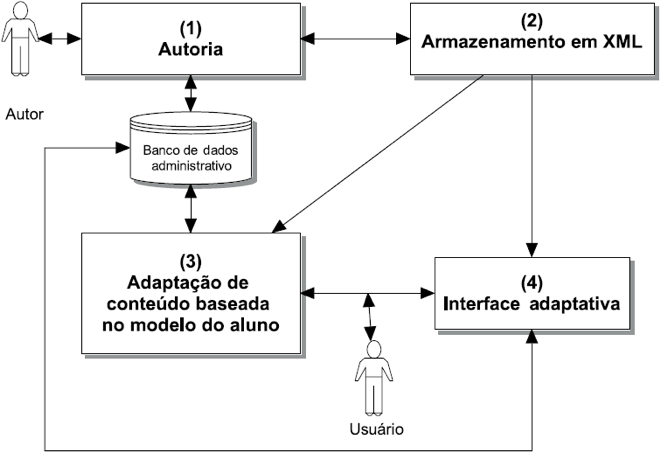
\includegraphics[scale=1.0]{./Figuras/adaptweb-arquitetura.png}
  \end{center}
  \legend{Fonte: \citeonline{gasparini2003interface}}
\end{figure}

O módulo de autoria (1) consiste na organização do conteúdo instrucional a ser disponibilizado para o aluno, sendo que
este conteúdo pode ter arquivos classificados como conceito, exemplos, exercícios e materiais complementares
\cite{gasparini2003interface}. Ao criar um conteúdo no sistema, o autor pode definir para quais cursos e disciplinas
deseja que o conteúdo ou arquivo esteja disponível. Isto significa que um aluno de um Curso X e de outro Curso Y,
matriculados em uma mesma disciplina, podem ter conteúdos distintos, conforme definido pelo professor. Por exemplo, a
disciplina de Cálculo I pode ser oferecida para os cursos de Ciência da Computação e Engenharia Elétrica e sua
abrangência e profundidade pode ser distinta para cada curso.

Em \citeonline{de2015sistema}, foi proposto uma nova categoria para os conteúdos chamada Links de Apoio. Esses Links de Apoio
são links externos ao ambiente \adaptweb que são cadastrados pelo professor como um
material alternativo de estudo e não estão diretamente atrelados á nenhum conceito em específico. O objetivo foi criar
uma nova categoria de materiais que poderia ser recomendada para o usuário a qualquer momento de sua interação.

O módulo de armazenamento em XML (2) é responsável por organizar os conteúdos e arquivos disponibilizados pelo autor em
um arquivo XML \cite{gasparini2003interface}. É utilizada a representação através de XML devido à sua alta
flexibilidade, oferecendo a estruturação dos documentos de forma independente da apresentação.

O módulo de adaptação do conteúdo baseado no modelo do aluno (3) é responsável por adaptar o conteúdo da disciplina
para cada curso. Por fim, o módulo de interface adaptativa (4) é responsável pela adaptação da navegação e da
apresentação da interface do ambiente de acordo com o curso, preferências do modo de navegação (modo tutorial ou livre)
e o conhecimento do usuário \cite{gasparini2003interface}.

\subsection{Sistema de Recomendação no \adaptweb}

Na Subseção \ref{subsection:estrutura-adaptweb} foi apresentada a estrutura do ambiente \adaptweb, que possui quatro categorias
de materiais para cada conteúdo. Além disso, existe uma outra categoria chamada Links de Apoio com o propósito de ser um
material auxiliar e que pode ser recomendado a qualquer momento para o usuário. Como no ambiente \adaptweb as palavras-chave para o itens
já são cadastradas pelo professor da disciplina, não será utilizada nenhuma técnica para captura automática das palavras-chave.

Fazendo uma relação da estrutura do \adaptweb com o algoritmo proposto no Capítulo \ref{chapter:proposta}, os itens de
todas as cinco categorias de materiais serão consideradas para a composição do perfil do usuário. Todos os
materiais acessados em cada uma das categorias é representado através das palavras-chave, e
essas palavras-chave farão parte do perfil do aluno a partir do momento em que este acessar o material. Já para os itens
recomendados, apenas os Links de Apoio serão considerados. O Sistema de Recomendação (SR) irá buscar, com
base nos itens acessados pelo aluno, os Links de Apoio mais adequados para a recomendação e irá apresentar através de uma
lista de itens. A forma de apresentação das Recomendações é discutida em mais detalhe na Subseção \ref{subsection:apresentacao-recomendacoes}.

\subsection{Apresentação das Recomendações}\label{subsection:apresentacao-recomendacoes}

A lista de recomendações neste trabalho será apresentada ao aluno na tela principal do ambiente do aluno. Dessa forma,
quando o SR possuir itens para recomendar para o usuário esses itens aparecem em uma lista logo abaixo do conteúdo que
ele estiver visualizando no momento, independente se o aluno esteja na tela de Conceito, Exercícios, Exemplos ou
Materiais Complementares. Na Figura \ref{fig:adaptweb-proposta-recomendacao} pode-se observar um protótipo da
apresentação das recomendações. Essas recomendações podem ser apresentadas ao usuário no momento em que este estiver acessando
quaisquer itens que sejam da categoria Conceito e Materiais Complementares, assim que o SR possuir itens relevantes para recomendar.

\begin{figure}[htb]
  \caption{\label{fig:adaptweb-proposta-recomendacao}Proposta de Interface de Recomendação}
  \begin{center}
      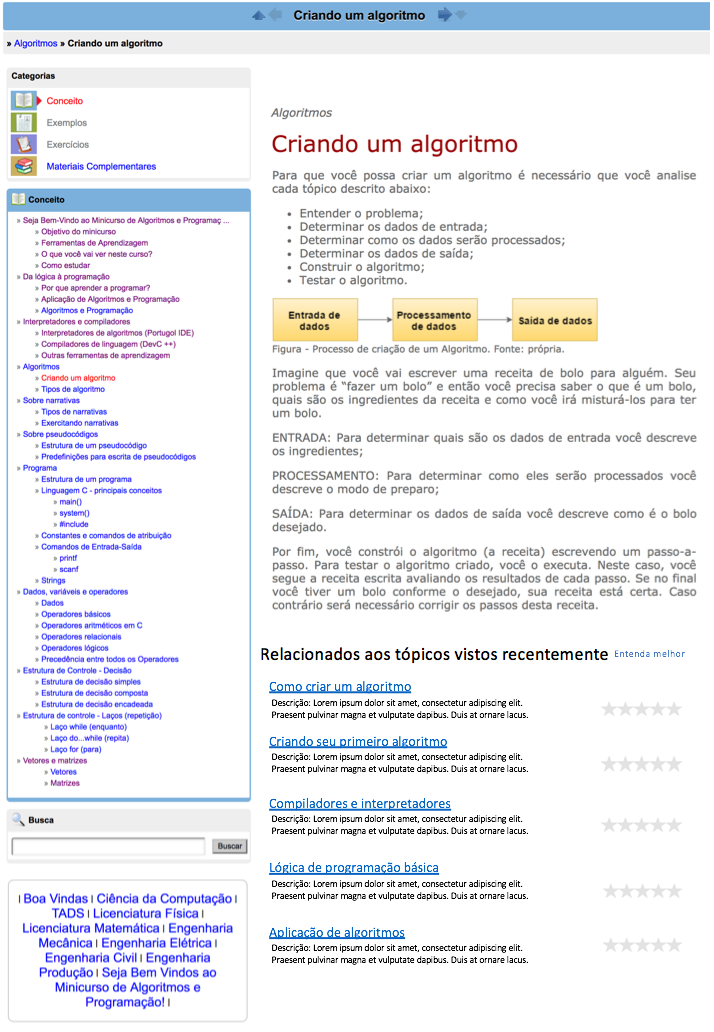
\includegraphics[scale=1.0]{./Figuras/recomendacoes_v2.png}
  \end{center}
  \legend{Fonte: O autor.}
\end{figure}

As principais informações dos Links de Apoio recomendados apresentados para o aluno são: Link, Nome do Link, Descrição e a possibilidade de avaliar o item
com notas de 1 a 5. A nota dada pelo usuário não será considerada pelo algoritmo em um primeiro momento, mas como trabalho
futuro pode vir a incorporar na recomendação, e.g., não tornar a recomendar itens que foram avaliado com notas baixas.
\citeonline{pu2012evaluating} afirmam que enquanto recomendar um item apenas é pouco, recomendar mais do que cinco itens
aumenta a dificuldade de escolhar do usuário. Por isso, a quantidade máxima de itens recomendadas para o usuário em cada
recomendação é de cinco itens.

Para cumprir o requisito de Explicação das recomendações citada por \citeonline{pu2012evaluating}, será adicionado um
botão de "Entenda melhor" que tem por objetivo explicar ao usuário como a lista de itens foi gerada. Ao entender o
funcionamento do algoritmo de recomendação o usuário tem a possibilidade aprimorar o seu perfil para personalizar as
recomendações recebidas. Na Figura \ref{fig:adaptweb-proposta-explicacao} está um protótipo da explicação da recomendação
mostrada para o aluno.

\begin{figure}[htb]
  \caption{\label{fig:adaptweb-proposta-explicacao}Explicação da recomendação}
  \begin{center}
      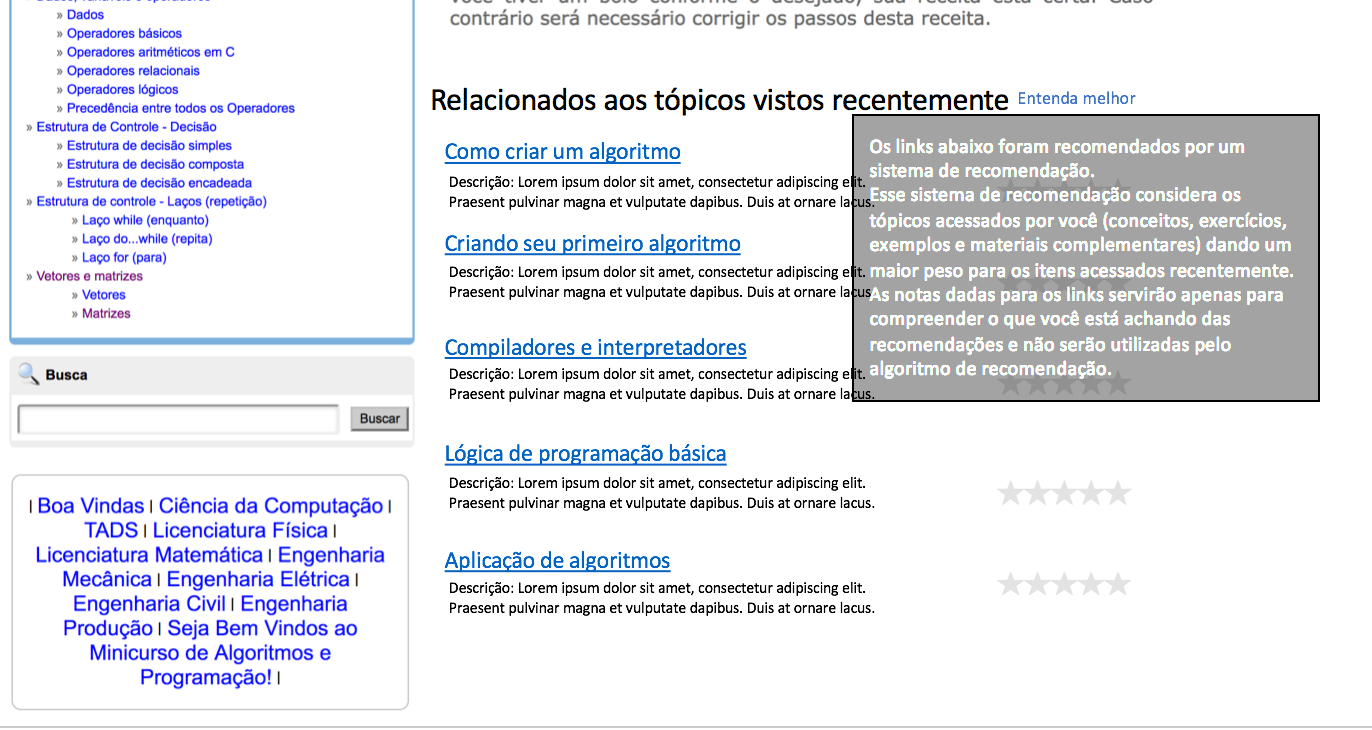
\includegraphics[scale=0.6]{./Figuras/explicacoes_v2.png}
  \end{center}
  \legend{Fonte: O autor.}
\end{figure}

\section{Definição do experimento}

O experimento proposto neste trabalho visa avaliar a experiência dos alunos ao interagir com o SR proposto, se comparado a um SR
utilizando a abordagem Baseada em Conteúdo tradicional. Este experimento foi
baseado nas seguintes hipóteses:

\begin{itemize}
\item \textbf{H\textsubscript{0}:} Não há diferenças na percepção do usuário da qualidade das recomendações recebidas utilizando a abordagem
Baseada em Conteúdo tradicional e a proposta desse trabalho.
\item \textbf{H\textsubscript{1}:} Há diferenças na percepção do usuário da qualidade das recomendações recebidas utilizando a abordagem
Baseada em Conteúdo tradicional e a proposta desse trabalho.
\end{itemize}

Para a execução do experimento, o SR proposto será comparado a abordagem Baseada em Conteúdo tradicional utilizando uma
estratégia \textit{Between Subjects}, i.e., os alunos serão divididos em dois grupos e cada grupo irá testar apenas
um dos sistemas. Porém, para garantir que a única variável será qual o SR utilizado, ambos os grupos irão utilizar a mesma
interface proposta para as recomendações.

O experimento será realizado em um minicurso de algoritmos do qual serão convidados a participar alunos de todos os cursos do Centro de
Ciências Tecnológicas (CCT) da Universidade do Estado de Santa Catarina (UDESC). Isso porque em todos os cursos do CCT
a disciplina de algoritmos está presente. O processo de design instrucional desse minicurso foi realizado por \citeonline{santos2017addie}.

Nesse minicurso costumam se matricular em média 100 alunos por semestre. Sendo que desses, espera-se que pelo menos 60 alunos chegam até
o final do curso e respondam ao questionário. Estima-se que o minicurso terá a duração de aproximadamente 45 dias e irá ocorrer no primeiro semestre
de 2018, entre os meses de Abril e Maio.

Os usuários ao se matricularem no minicurso serão aleatóriamente divididos nos dois grupos de usuários, de forma que ambos
os grupos tenham uma quantidade de usuários similar. Além disso, os alunos irão receber um Termo de Consentimento Livre
e Esclarecido (TCLE) que explica o objetivo do experimento e no qual eles irão consentir em participar dos experimentos e
em permitir o uso dos resultados do experimento para essa pesquisa, sempre garantindo a anonimidade dos participants.

Ao final dos 45 dias do minicurso, os alunos irão receber um questionário para responder sobre a sua experiência com o SR.
Esse questionário será produzindo utilizando um subconjunto das perguntas definidas por \citeonline{pu2011user} (presente no
Anexo \ref{ane:questoes-framework}), que deverão ser traduzidas para o português para garantir o entendimento de todos os alunos.
Os resultados dos questionários serão  analisados através de métodos estatísticos para definir se existe diferença
significativa entre a percepção do usuário da qualidade das recomendações nos dois SRs (o proposto e o Baseado em Conteúdo tradicional) e, se existir,
qual deles teve o melhor desempenho.

\section{Teste piloto}

Antes do experimento ser realizado com os alunos das disciplinas de algoritmos do CCT, será realizado um teste piloto com
outros alunos da universidade que já realizaram essa disciplina. O objetivo desse teste piloto será avaliar os
instrumentos do experimento, além de permitir encontrar problemas na experiência do  usuário para serem corrigidos
antes da execução do minicurso.

Para o teste piloto, os alunos receberão o TCLE ao qual eles também serão pedidos a assinar e serão pedidos a realizar algumas
tarefas dentro do minicurso de algoritmos enquanto são observados por um pesquisador. As tarefas envolverão o acesso a
alguns conceitos, exemplos, exercícios e materiais complementares, como também a ferramenta de recomendação. Ao final, os
participantes do teste piloto irão responder ao questionário desenvolvido (o mesmo que será aplicado no experimento) e
serão entrevistados pelo pesquisador sobre problemas encontrados nos instrumentos.

Com o resultado da observação do pesquisador e do questionário respondido pelos participantes do teste piloto será possível
identificar possíveis problemas no sistema desenvolvido para serem corrigidos antes da execução do experimento. Já o objetivo da
entrevista será exclusivamente para aprimorar os instrumentos (i.e., TCLE e o questionário desenvolvido).

\section{Considerações sobre o capítulo}

Neste capítulo foi descrito o ambiente no qual o Sistema de Recomendação (SR) proposto será incorporado (\adaptweb) e definido o
experimento para a avaliação da proposta desse trabalho. Nos SRs desenvolvidos no \adaptweb, tanto para a proposta deste trabalho como para a abordagem
Baseada em Conteúdo tradicional que será utilizada como parâmetro, o perfil do usuário é composto pelo conjunto de palavras-chave de todos os itens acessados pelo usuário, das
cinco categorias apresentadas. Os itens a serem recomendados são os Links de Apoio, visto que os itens das outras categorias
são estruturados pelo professor e estão fortemente relacionados à conceitos específicos.

Utilizando como base as diretrizes propostas por \citeonline{pu2012evaluating} foi proposta uma interface para a apresentação das recomendações no \adaptweb,
com o objetivo de que os usuários tenham acesso direto as recomendações na tela principal do ambiente do aluno e entendam
melhor o porque aqueles itens foram recomendados. Como visto, essa interface será utilizada tanto pelo algoritmo proposto
quanto pela abordagem tradicional.

O experimento visa avaliar a experiência do usuário com o SR proposto no Capítulo \ref{chapter:proposta} em
comparação à abordagem Baseada em Conteúdo tradicional. O experimento acontecerá no ambiente
\adaptweb através de um minicurso de algoritmos desenvolvido no ambiente nos meses de
Abril e Maio de 2018. Ao final do minicurso os alunos receberão um questionário para responder sobre a sua experiência
ao interagir com o SR, que será adaptado do conjunto de questões definidas por \citeonline{pu2011user}. Ao final do
experimento, espera-se chegar a uma conclusão se existe diferença na percepção do usuário sobre a qualidade
das recomendações recebidas ao utilizar um SR Sensível ao Tempo, que se adapta as variações de interesse do
aluno, em relação a uma abordagem tradicional de recomendação.
